%% Modelo de relatório para trabalhos do Instituto Federal do Ceará
%% Felipe José de Sousa Vasconcelos, felipe.vasconcelos@ifce.edu.br

\documentclass[
	% -- opções da classe memoir --
	12pt,				% tamanho da fonte
	openany,
% 	openright,			% capítulos começam em pág ímpar (insere página vazia caso preciso)
% 	twoside,			% para impressão em recto e verso. Oposto a oneside
    oneside,			% para impressão em recto e verso. Oposto a oneside
	a4paper,			% tamanho do papel. 
	% -- opções da classe abntex2 --
	chapter=TITLE,		% títulos de capítulos convertidos em letras maiúsculas
	%section=TITLE,		% títulos de seções convertidos em letras maiúsculas
	%subsection=TITLE,	% títulos de subseções convertidos em letras maiúsculas
	%subsubsection=TITLE,% títulos de subsubseções convertidos em letras maiúsculas
	% -- opções do pacote babel --
	%brazil,			    % idioma adicional para hifenização
	french,				% idioma adicional para hifenização
	spanish,			% idioma adicional para hifenização
	english				% o último idioma é o principal do documento
	]{ifce-relatorio-abntex2}

% ---
% Pacotes básicos 
% ---
\usepackage{mathptmx}			% Usa a fonte Times New Roman para texto e equações
\usepackage[T1]{fontenc}		% Selecao de codigos de fonte.
\usepackage[utf8]{inputenc}		% Codificacao do documento (conversão automática dos acentos)
\usepackage{lastpage}			% Usado pela Ficha catalográfica
\usepackage{indentfirst}		% Indenta o primeiro parágrafo de cada seção.
\usepackage{color}				% Controle das cores
\usepackage{graphicx}			% Inclusão de gráficos
\usepackage{microtype} 			% para melhorias de justificação
%\usepackage{pdfpages}			% adiciona páginas em pdf no texto
% ---
		
% ---
% Pacotes adicionais, usados apenas no âmbito do Modelo Canônico do abnteX2
% ---
\usepackage{lipsum}				% para geração de dummy text
% ---

% ---
% Pacotes de citações
% ---
\usepackage[english,hyperpageref]{backref}	 % Paginas com as citações na bibl
\usepackage[alf]{abntex2cite}	% Citações padrão ABNT

% ---
% Pacotes do usuário
% ---
%\usepackage[capposition=top]{floatrow}
\usepackage{caption}			% Edita propriedades de legendas de figuras e tabelas
% \usepackage[fleqn]{amsmath}		% Alinha à esquerda todas as equações
% \setlength{\mathindent}{0pt}	% Alinha à esquerda todas as equações
\graphicspath{{Figures/}}
\usepackage{mathtools}			% Equações condicionais
\usepackage{tikz}
\usepackage{xcolor}
\usetikzlibrary{shapes,arrows}
\usepgflibrary{arrows.meta}
\usepackage[position=bottom]{subfig}
\usepackage{psfrag}
\usepackage{amsmath,amsfonts,float,bm}
\usepackage{latexsym,amssymb,array}

% --- 
% CONFIGURAÇÕES DE PACOTES
% --- 

% ---
% Configurações do pacote backref
% Usado sem a opção hyperpageref de backref
\renewcommand{\backrefpagesname}{Citado na(s) página(s):~}
% Texto padrão antes do número das páginas
\renewcommand{\backref}{}
% Define os textos da citação
\renewcommand*{\backrefalt}[4]{
	\ifcase #1 %
		Nenhuma citação no texto.%
	\or
		Citado na página #2.%
	\else
		Citado #1 vezes nas páginas #2.%
	\fi}%
% ---

% ---
% Informações de dados para CAPA e FOLHA DE ROSTO
% ---
\instituicao{
Instituto Federal de Educação, Ciência e Tecnologia do Ceará
\protect\\
Departamento da Indústria
\protect\\
Programa de graduação em Engenharia Elétrica}
\titulo{Disciplina}
\subtitulo{Título do relatório}
\local{Cidade}
% data da defesa
\dia{xx}
\mes{xx}
\ano{ANO}
\diamesano{\imprimirmes~\imprimirdia, \imprimirano}
\data{\imprimirano}
% %
\newcommand{\definirautores}{%
    \autor{%
            Alunos\qquad\qquad\= Nome do Aluno 1 - 12345\\
                     \> Nome do Aluno 2 - 12345\\
                     \> Nome do Aluno 3 - 12345\\
                     \> Nome do Aluno 4 - 12345\\
            Professor\> Nome do Professor 
    }
}
\definirautores
% \autor{}

% ---
% Configurações de aparência do PDF final

% alterando o aspecto da cor azul
\definecolor{blue}{RGB}{41,5,195}

% informações do PDF
\makeatletter
\hypersetup{
     	%pagebackref=true,
		pdftitle={\@title}, 
		pdfauthor={\@author},
    	% pdfsubject={\imprimirpreambulo},
	    pdfcreator={LaTeX with abnTeX2},
		pdfkeywords={abnt}{latex}{abntex}{abntex2}{trabalho acadêmico}, 
		colorlinks=true,       		% false: boxed links; true: colored links
    	linkcolor=blue,          	% color of internal links
    	citecolor=blue,        		% color of links to bibliography
    	filecolor=magenta,      	% color of file links
		urlcolor=blue,
		bookmarksdepth=4
}
\makeatother
% --- 

% --- 
% Espaçamentos entre linhas e parágrafos 
% --- 

% O tamanho do parágrafo é dado por:
\setlength{\parindent}{1.3cm}

% Controle do espaçamento entre um parágrafo e outro:
\setlength{\parskip}{0.2cm}  % tente também \onelineskip

% ---
% compila o indice
% ---
\makeindex
% ---

\begin{document}
% Seleciona o idioma do documento (conforme pacotes do babel)
\selectlanguage{brazil}

% Retira espaço extra obsoleto entre as frases.
\frenchspacing 

% ----------------------------------------------------------
% ELEMENTOS PRÉ-TEXTUAIS
% ----------------------------------------------------------
% \pretextual

% ---
% Capa
% ---
\imprimircapa
% ---

% ---
% inserir o sumario
% ---
\pdfbookmark[0]{\contentsname}{toc}
\tableofcontents*
\cleardoublepage
% ---

% ----------------------------------------------------------
% ELEMENTOS TEXTUAIS
% ----------------------------------------------------------
\textual

% ----------------------------------------------------------
% Introdução
% ----------------------------------------------------------
\chapter{Introdução} \label{ch:intro}
% ----------------------------------------------------------
\textcolor{red}{Lembre-se sempre de utilizar labels adequadas!}

\lipsum[2-2]

\section{Objetivos} \label{sec:obj}
Esse é um exemplo de seção. A seguir um exemplo de subseção.

\subsection{Objetivos específicos} \label{subsec:objEspec}
Ainda é possível utilizar uma sub-subseção. 

\subsubsection{Separando objetivos específicos} \label{subsubsec:sep_objEspec}

% ----------------------------------------------------------
% Desenvolvimento e Metodologia
% ----------------------------------------------------------
\chapter{Desenvolvimento e Metodologia} \label{ch:metodos}
% ----------------------------------------------------------
\lipsum[2-3]

\section{Inserindo equações e figuras} \label{sec:Eq_fig}

 Equações podem ser escritas nos mais diversos ambientes. Pode-se simplesmente utilizar o ambiente matemático inserindo a equação entre cifrões $x=a+b$, como também é possível utilizar ambientes próprios:
 \begin{equation} \label{eq:eq_simples}
     x^2+2x+3=y.
 \end{equation}
 
 Caso seja necessário escrever um conjunto de equações:
  \begin{eqnarray} \label{eq:eq_composta1}
     x^2+2x+3=y\\
     x^2+2x+3=y,
 \end{eqnarray}
 \noindent
 a equação \eqref{eq:eq_composta1} pode também ser escrita com o ambiente:
  \begin{align} \label{eq:eq_composta2}
     x^2+2x+3&=y\\
     x^2+2x+3&=y,
  \end{align}
\noindent
contudo, caso não seja necessário numerar a equação basta fazer:
  \begin{align*} 
     x^2+2x+3&=y\\
     x^2+2x+3&=y.
  \end{align*}

Também é possível escrever matrizes:
\begin{align} \label{eq:ex_matriz}
    A = \left[\begin{array}{cc}
        a & b\\
        c & d
    \end{array}\right]
\end{align}
\noindent

A forma mais simples de inserir figuras é por meio do ambiente (são aceitos diversos formatos como jpeg, png, eps, pdf, etc):
\begin{figure}[H]
    \centering
    \caption{Este é um exemplo de figura.}
    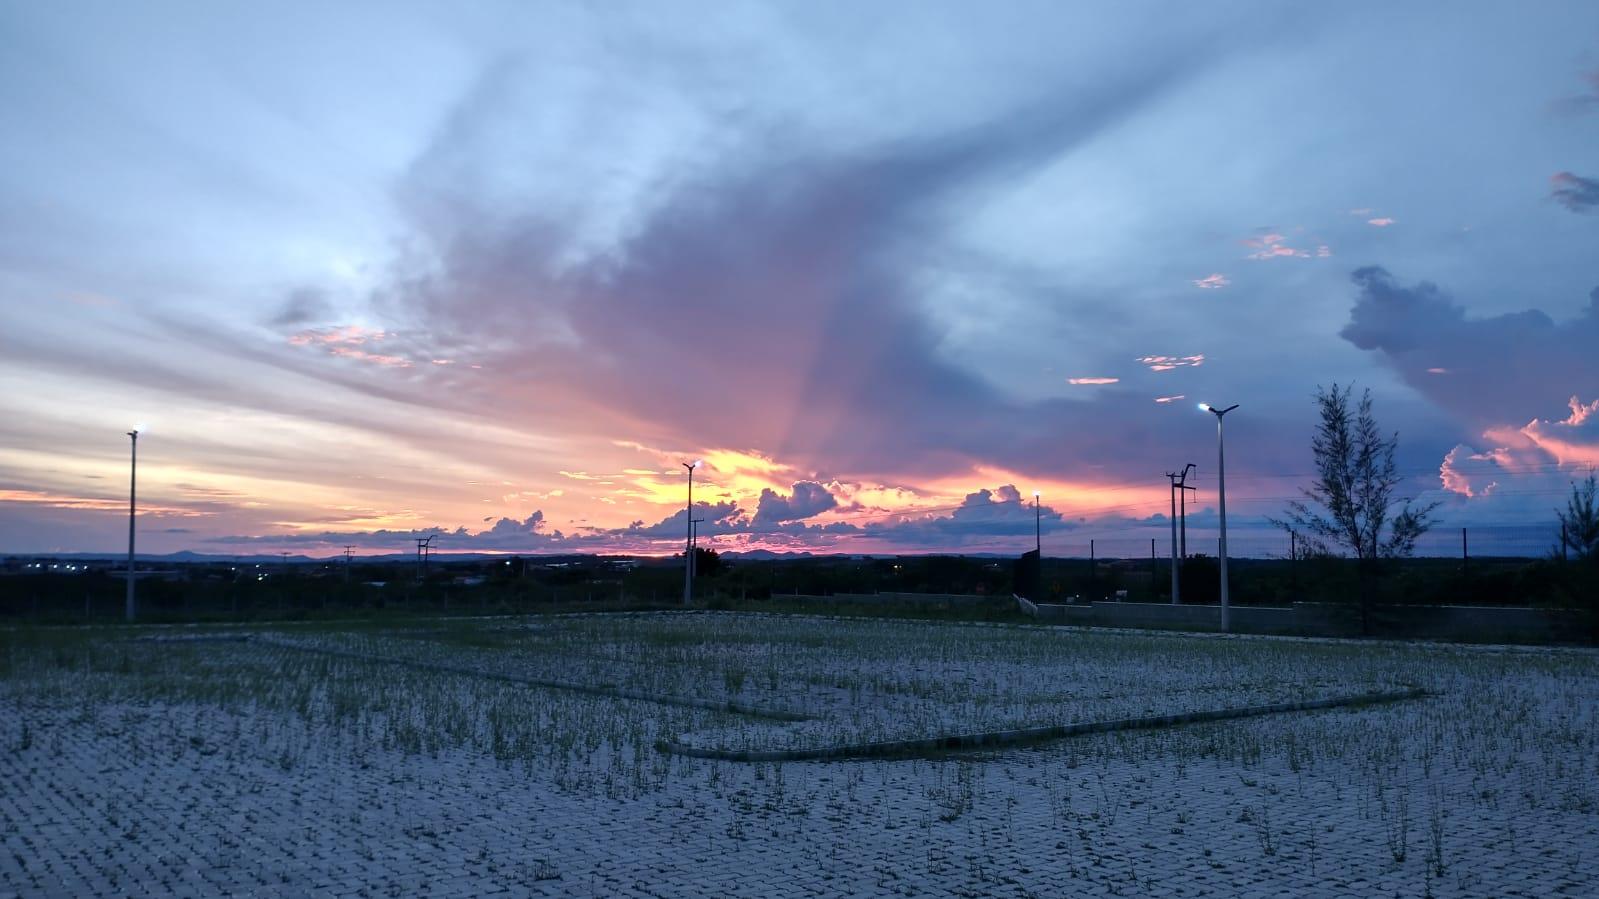
\includegraphics[scale=0.2]{Figuras/por_do_sol.jpeg}
	\captionsetup{font=small}
	\caption*{Fonte: Autor.}
    \label{fig:por_do_sol}
\end{figure}

Na Figura \ref{fig:por_do_sol} é utilizada uma imagem simples, mas também é possível inserir mais de uma imagem, bastando utilizar bibliotecas apropriadas.
  
% ----------------------------------------------------------
% Procedimento experimental
% ----------------------------------------------------------
\chapter{Procedimento experimental} \label{ch:proced}
% ----------------------------------------------------------

\section{Equipamentos utilizados} \label{sec:equip}

Citações indiretas podem ser feitas dessa forma \cite{lathi2006sinais}. Contudo para citações diretas use conforme sugerido em \citeonline{franklin2013sistemas}.

\section{Inserindo tabelas} \label{sec:tab}

Para escrever tabelas sugere-se o site: \href{https://www.tablesgenerator.com}{Tables generator}. Um exemplo de tabela:
\begin{table}[H]%[!htb]
    \centering
    \caption{Exemplo de tabela.}
    \begin{tabular}{ccc}
    \hline
    Índice 1 & Índice 2 & Índice 3 \\ \hline
    1 & 2 & 3 \\
    4 & 5 & 6 \\ \hline
    \end{tabular}
     \label{tab:tabela_indices}
\end{table}

% ----------------------------------------------------------
% Conclusões
% ----------------------------------------------------------
\chapter{Conclusões} \label{ch:conclusao}
% ----------------------------------------------------------

\lipsum[2-3]

% ----------------------------------------------------------
% ELEMENTOS PÓS-TEXTUAIS
% ----------------------------------------------------------
% \postextual
% ----------------------------------------------------------

% ----------------------------------------------------------
% Referências bibliográficas
% ----------------------------------------------------------
\bibliography{referencias}

\end{document}